\documentclass[conference]{IEEEtran}
\IEEEoverridecommandlockouts
\usepackage[utf8]{inputenc}
\usepackage[T1]{fontenc}
\usepackage{cite}
\usepackage{amsmath,amssymb}
\usepackage{graphicx}
\usepackage{booktabs}
\usepackage{url}
\usepackage[hidelinks]{hyperref}
\graphicspath{{../../reports/figures/}{../}{../../reports/experiments/}}

\begin{document}

\title{TRM Predict: A Cloud-Native Predictive Analytics System for Exchange-Rate Risk Decisions in Colombia}

\author{
\IEEEauthorblockN{Sebastián Cubides, Nicolás Vergara, Edgar Ruiz}
\IEEEauthorblockA{\textit{Data Engineering and Artificial Intelligence, 5th semester}\\
\textit{Universidad Santo Tomás}, Tunja, Colombia\\
Integrative Project: Data Mining, Machine Learning and Cloud Computing --- 2026-2}
}

\maketitle

\begin{abstract}
Households that receive remittances and micro, small and medium enterprises (MSMEs) that import goods in Colombia are exposed to the volatility of the peso--dollar exchange rate (TRM) without the analytical tools of large firms. We present \emph{TRM Predict}, a cloud-native decision-support system that forecasts, for the next business day, the direction of the TRM, its expected value and the probability of a large move. A CRISP-DM pipeline integrates the official TRM, eight market series, two crypto-assets and a web-scraped news-sentiment index into a leakage-free data set of 2{,}159 days and 43 features. Unsupervised mining identifies three market regimes, 57 anomalous days and association rules with lift up to 1.24. Among 19 tuned models, only the ensembles beat chance out of sample: Gradient Boosting reaches a test ROC-AUC of 0.566 for direction and 0.586 for risk, and a regression RMSE 2.4\% below the random walk; a remittance-household simulation turns the direction signal into a positive gain versus always selling at once. The system runs on AWS and is fully described in Terraform (64 resources): serverless ingestion, an S3 data lake replicated across regions, PostgreSQL on RDS and a containerized API behind a load balancer with auto-scaling in two availability zones. Experiments show that, with at least one instance per zone, terminating a server causes no failed request (100\% availability versus 77.8\% with a single minimum instance), and that scaling out from two to four instances raises throughput by 84\% and cuts median latency by 60\%. The project contributes to SDG~8 (target 8.10) and SDG~10 (target 10.c).
\end{abstract}

\begin{IEEEkeywords}
cloud computing, data mining, machine learning, CRISP-DM, ensemble learning, exchange-rate forecasting, infrastructure as code, sustainable development
\end{IEEEkeywords}

\section{Introduction}
The \emph{Tasa Representativa del Mercado} (TRM) is the official COP/USD exchange rate certified every day by Colombia's Financial Superintendence. It sets the price of imported goods, the value of the remittances received by households and the cost of dollar-denominated debt. Between September 2017 and October 2026 it moved between 2{,}705 (April 2018) and 5{,}061 COP/USD (November 2022); during 2025 alone it ranged from 3{,}707 to 4{,}417, a 19\% swing, and 18\% of trading days in our sample show a variation larger than 1\%.

Large firms hedge this risk with treasury desks and derivatives, whereas households and MSMEs usually decide by intuition. Remittances to Colombia exceeded USD~11.8 billion in 2024~\cite{banrep_remesas}, so a better choice of \emph{when} to convert dollars has a tangible effect on family income. The project therefore addresses the 2030 Agenda~\cite{un2015}: SDG~8 (target 8.10, access to financial services) and SDG~10 (target 10.c, reducing the cost of remittances).

\textbf{Contributions.} (i) A reproducible KDD/CRISP-DM pipeline over heterogeneous public sources, including a purpose-built web scraper; (ii) an honest benchmark of 19 regression and classification models against random-walk and majority-class baselines, with SHAP and LIME explanations and a decision-oriented evaluation; (iii) a production-style AWS deployment written entirely as Infrastructure as Code, with measured scalability, availability and cost.

\section{Problem Statement}
\textbf{Users.} Households receiving remittances, importing MSMEs, and financial-literacy programs. \textbf{Question.} Using only public data available before the next TRM is published, can we estimate (a) the probability that it rises, (b) its expected value and (c) the probability of an abnormally large move, verifiably better than naive baselines, and explain each prediction? Exchange rates are notoriously hard to forecast: Meese and Rogoff showed that structural models fail to beat a random walk out of sample~\cite{meese1983}. Consequently, the random walk and the majority class are mandatory baselines in this work.

\section{Related Work}
Henrique \emph{et al.}~\cite{henrique2019} review machine learning for financial-market prediction and report the dominance of support vector machines and neural networks, with ensembles gaining ground; Sezer \emph{et al.}~\cite{sezer2020} survey deep learning for financial time series and stress its weak interpretability and reproducibility. Most studies address major currency pairs or equity indices and stop at offline evaluation. This work targets an emerging-market currency, uses country-specific drivers (oil, peer currencies, local news), favors interpretable ensembles explained with SHAP~\cite{lundberg2017} and LIME~\cite{ribeiro2016}, and delivers a deployed, reproducible service.

\section{System Overview}
Fig.~\ref{fig:arch} depicts the system. Every business day at 18:30 (Colombia time), an EventBridge rule triggers the \emph{ingestion} Lambda, which calls the TRM open-data API, Yahoo Finance and Binance, scrapes \emph{La Rep\'ublica}, and writes one JSON bundle to the raw zone of an S3 data lake. That object triggers the \emph{ETL} Lambda, which upserts the data into PostgreSQL. Models are trained offline with the pipeline described below and published to S3. A FastAPI service in Docker serves predictions, what-if scenarios and a web dashboard (Fig.~\ref{fig:dash}).

\begin{figure*}[t]
\centering
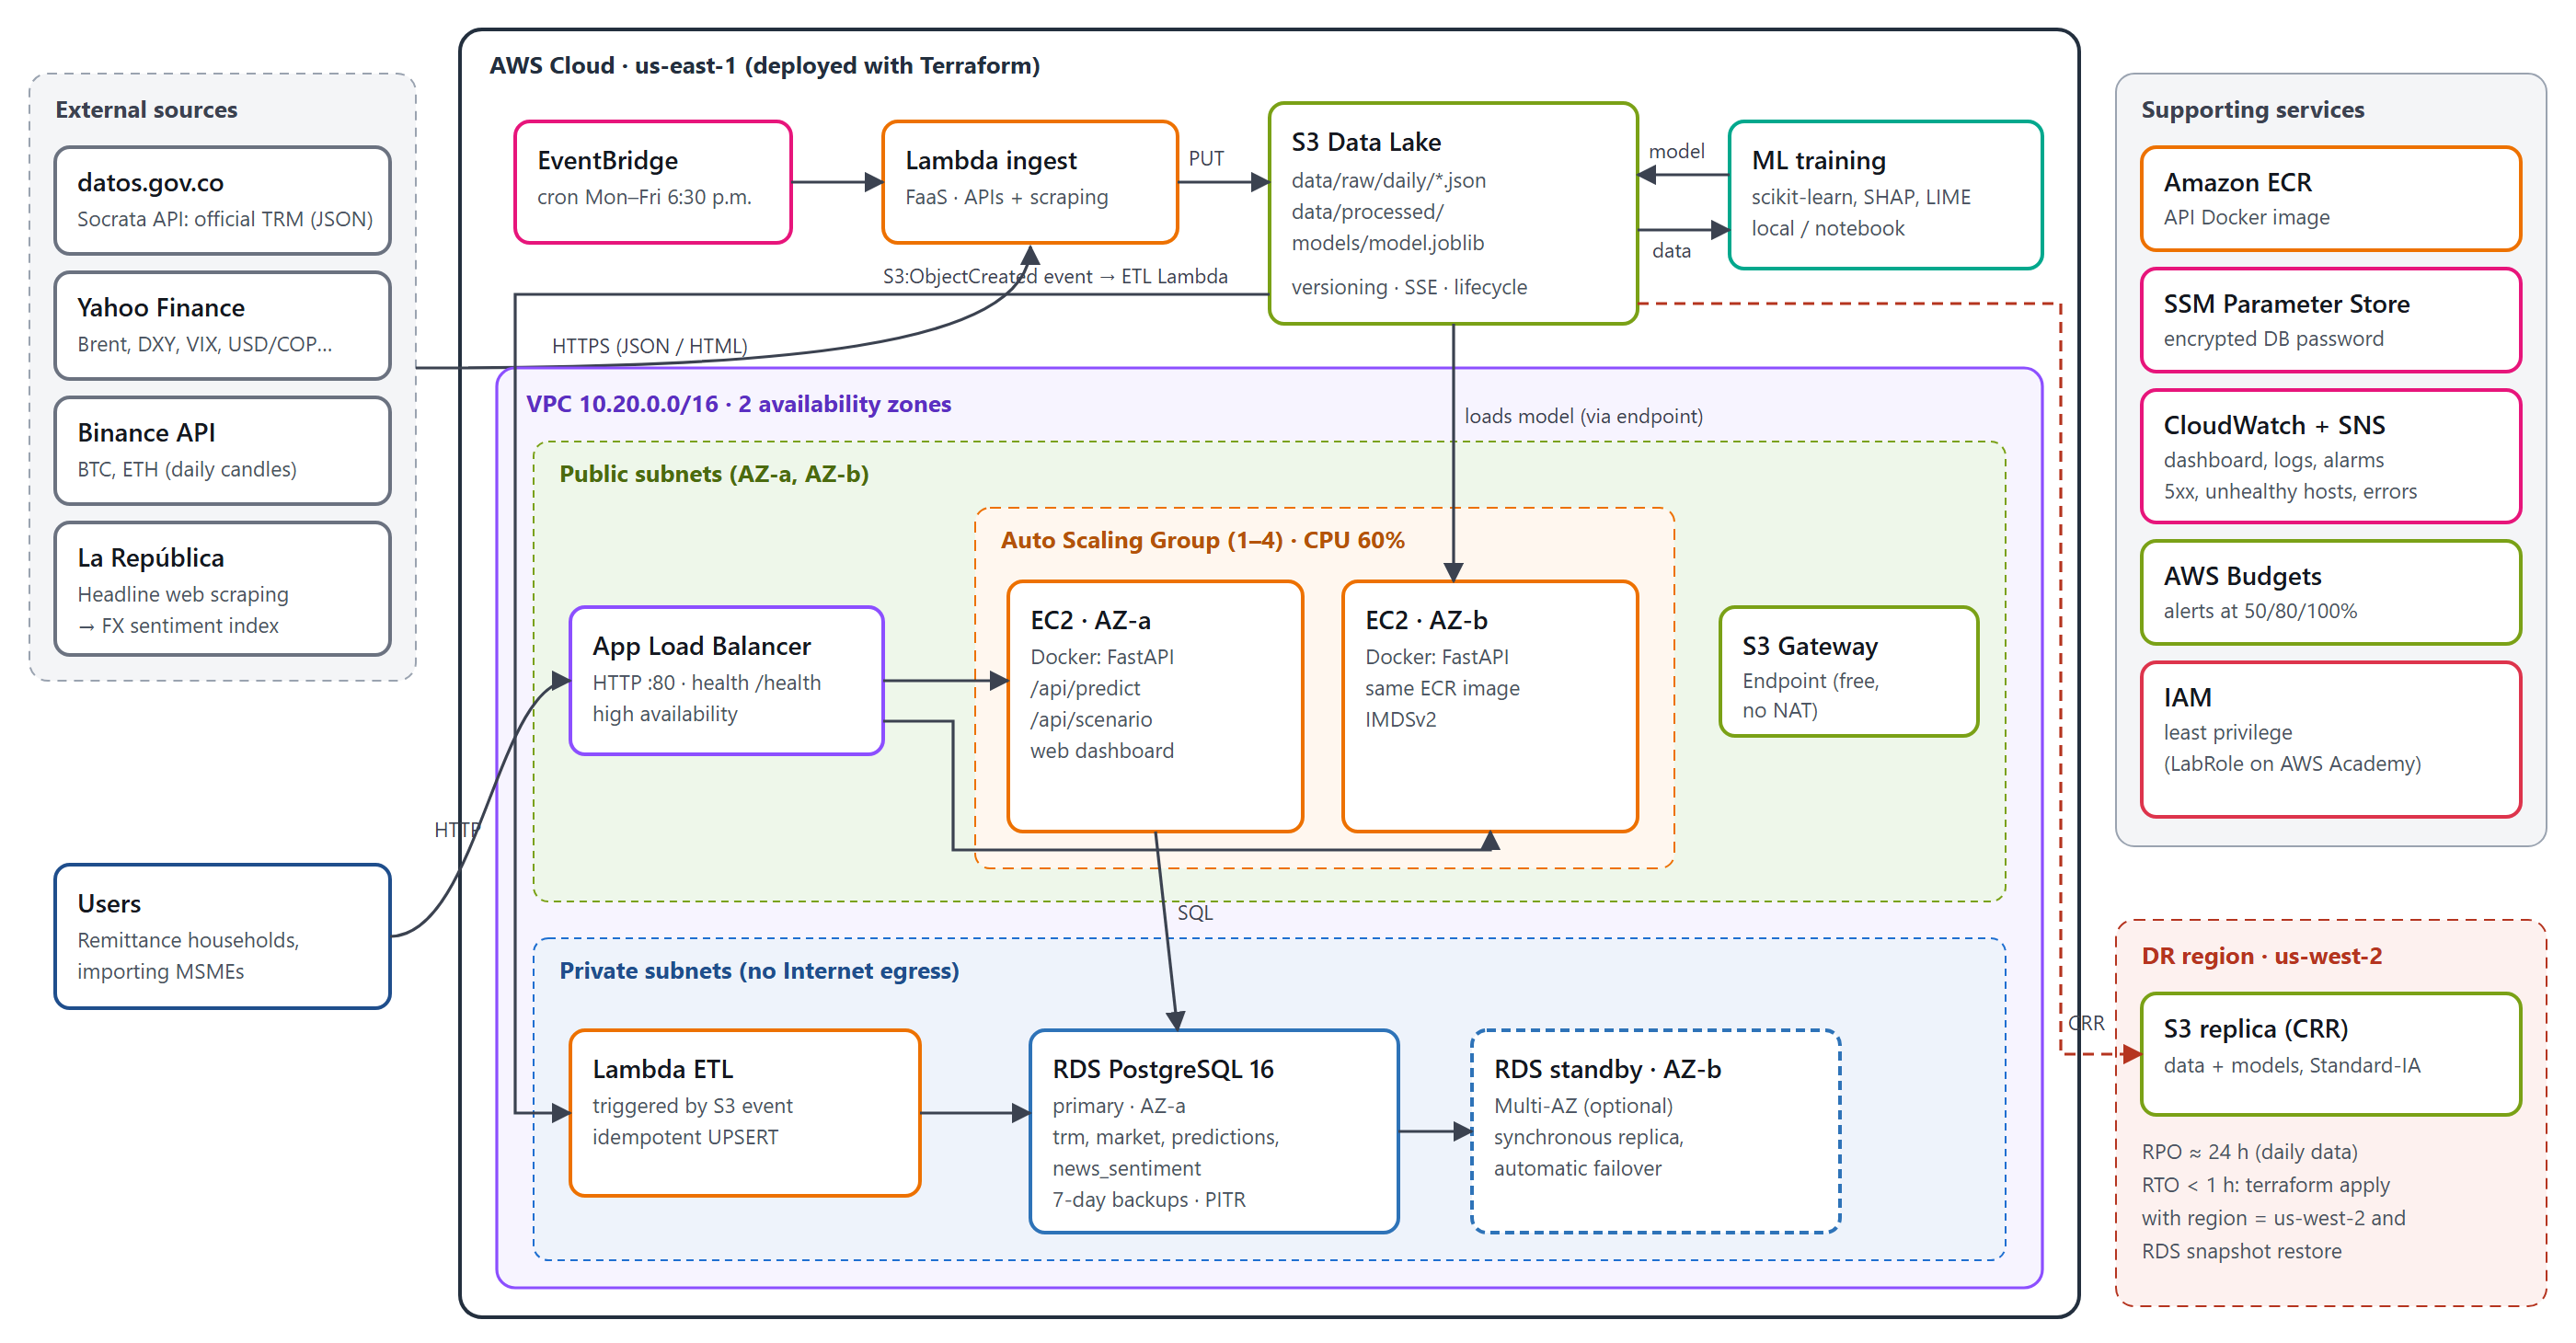
\includegraphics[width=0.95\textwidth]{arquitectura_en.png}
\caption{TRM Predict architecture on AWS, deployed with Terraform.}
\label{fig:arch}
\end{figure*}

\section{Data Mining Pipeline}
The pipeline follows the KDD process~\cite{fayyad1996} organized with CRISP-DM~\cite{wirth2000}; every stage is a Python module that can be re-run end to end.

\subsection{Data Acquisition}
Table~\ref{tab:sources} lists the sources. The scraper has a specific function that no API covers: it collects the headlines of three sections of \emph{La Rep\'ublica}, counts those about the dollar and computes a lexicon-based FX-sentiment score ($-1$ to $1$). It uses only the Python standard library so that it runs inside Lambda, issues one request per section per day and isolates its failures from numeric ingestion. Because historical headlines are not available, the score is stored daily and shown in the dashboard; it will enter the models once enough history accumulates.

\begin{table}[t]
\caption{Data sources}
\label{tab:sources}
\centering
\footnotesize
\begin{tabular}{@{}p{2.1cm}p{1.4cm}p{3.9cm}@{}}
\toprule
Source & Format & Content \\
\midrule
datos.gov.co (Superfinanciera) & API, JSON & Official TRM since 1991 (8{,}370 records) \\
Yahoo Finance & API, JSON$\to$CSV & Brent, DXY, US 10Y, VIX, S\&P 500, USD/MXN, USD/BRL, USD/COP spot \\
Binance (data-api) & API, JSON$\to$CSV & BTC and ETH daily candles \\
La Rep\'ublica & HTML scraping & Headlines and FX-sentiment index \\
\bottomrule
\end{tabular}
\end{table}

\subsection{Preparation and Data Quality}
Cleaning includes type casting, removal of duplicates and invalid dates, positivity checks and an audit of outlying returns with the $3\times$IQR rule (e.g., 61 for Brent and 44 for the US 10Y yield; they are genuine market events and were kept, as tree ensembles are robust to them). Integration uses a strict \texttt{merge\_asof} with \texttt{allow\_exact\_matches=False}: for the TRM valid on day $d$, only market closes \emph{before} $d$ are used, which prevents look-ahead leakage. The final data set has 2{,}159 days (Sep.~2017--Oct.~2026), constrained by the start of the crypto series, and 43 features (TRM log-returns and lags, 5/20-day volatility, moving-average ratio, z-score, calendar; 1/5-day returns and 20-day volatility of each market; and the spot--TRM gap). Targets are the next log-return $y_{ret}$, its sign $y_{up}$ and a large-move flag $y_{big}=\mathbb{1}[|y_{ret}|>q_{75}]$, with $q_{75}=0.86\%$ computed on the training set only.

\subsection{Exploratory Data Analysis}
TRM returns are leptokurtic (excess kurtosis 3.0, skewness 0.50, Jarque--Bera $p<10^{-100}$) and show positive lag-1 autocorrelation (0.17), consistent with the TRM being a volume-weighted daily average. Only 48.3\% of days are up-moves. The variables most correlated with the next return are the last TRM return (0.17), Brent (0.13) and the DXY (0.09). Rolling correlations (Fig.~\ref{fig:eda}) reveal that these relations change sign over time, which anticipates the low out-of-sample predictability.

\begin{figure}[t]
\centering
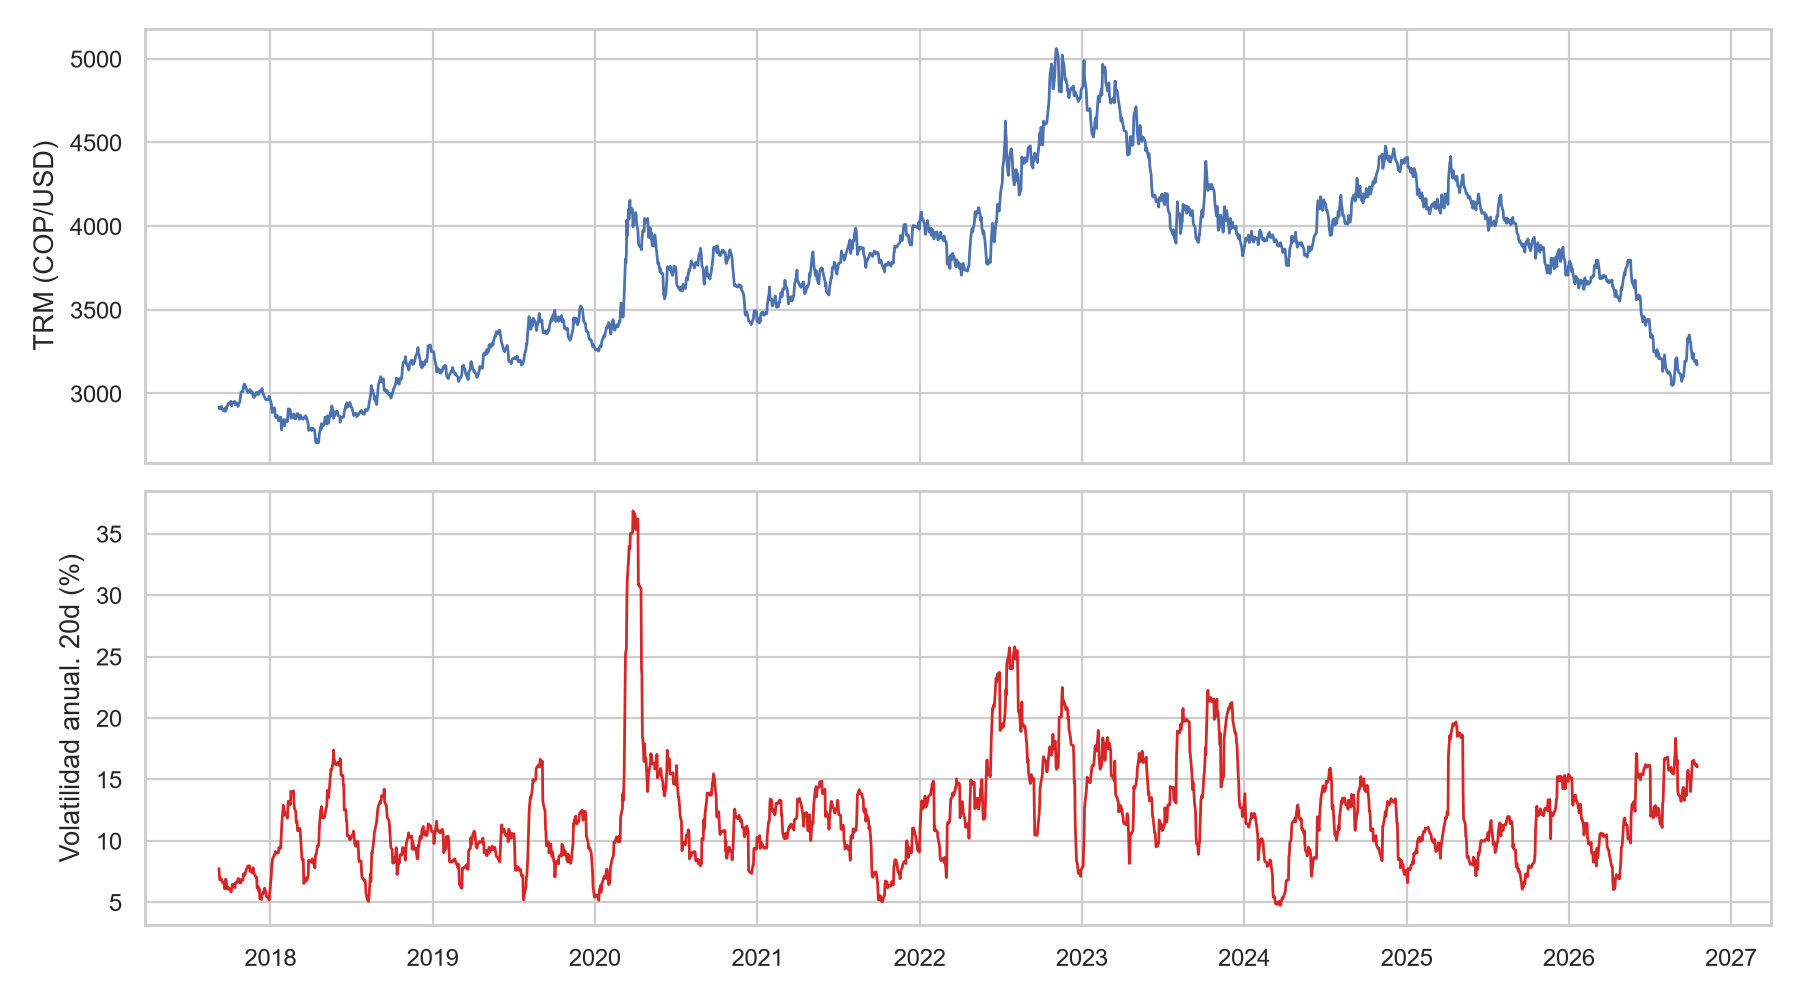
\includegraphics[width=\columnwidth]{eda_trm_series.png}\\[2pt]
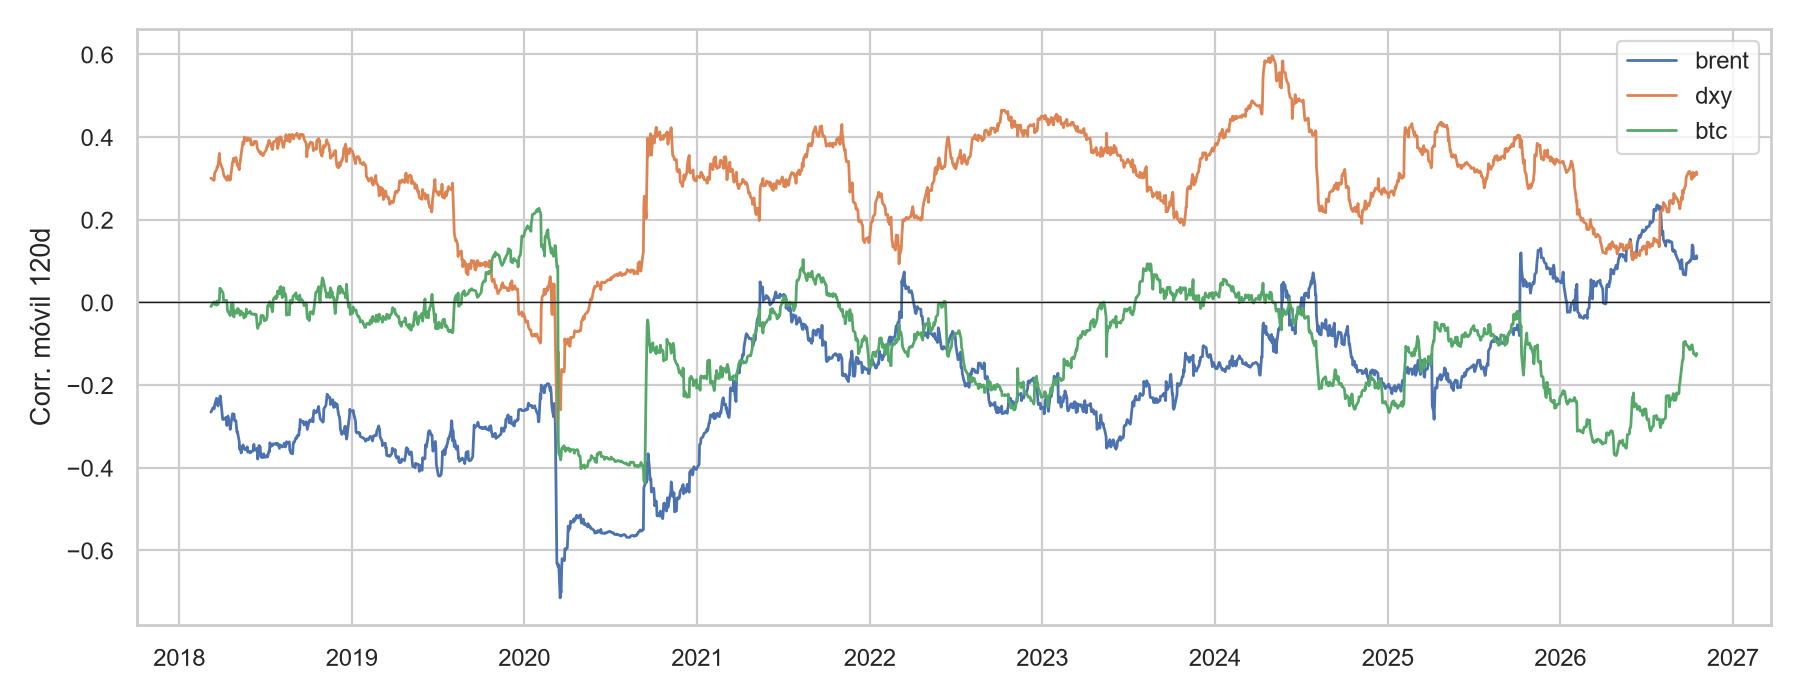
\includegraphics[width=\columnwidth]{eda_rolling_corr.png}
\caption{TRM level and 20-day annualized volatility (top) and 120-day rolling correlation between the TRM and Brent, DXY and BTC (bottom).}
\label{fig:eda}
\end{figure}

\subsection{Feature Engineering and PCA}
PCA on standardized features needs 26 of 43 components to retain 90\% of the variance, so the features are only weakly redundant and dimensionality reduction would discard information; it is used for analysis and visualization only. PC1 loads on peso and peer-currency momentum (5-day TRM return, USD/COP, USD/MXN, z-score), and PC2 on global volatility (S\&P~500, US~10Y, Brent, DXY).

\subsection{Clustering: Market Regimes}
Nine regime features (volatility and 5-day momentum of the TRM, VIX, DXY, Brent, BTC and S\&P~500) were standardized. With raw data, K-Means at $k=2$ only isolates the 33 most extreme days of 2020; tails were therefore clipped to the 1st--99th percentiles before K-Means and Ward hierarchical clustering, whereas DBSCAN~\cite{ester1996} was applied to the unclipped data as an anomaly detector. The silhouette method selects $k=3$ for both algorithms (Table~\ref{tab:regimes}): a risk-off regime in which the TRM rises on 52.9\% of the next days, a risk-on regime (44.3\%) and a high-volatility regime whose next-day volatility is 1.7 times higher. The low silhouette (0.12; Davies--Bouldin 2.08) shows overlapping regimes, which are thus used as context rather than as hard classes. DBSCAN ($\varepsilon=2.89$ from the 95th percentile of the 18-distance curve, \texttt{min\_samples}=18) flags 57 anomalous days (45 in 2020), on which next-day volatility is 1.73 times that of normal days.

\begin{table}[t]
\caption{K-Means market regimes ($k=3$)}
\label{tab:regimes}
\centering
\footnotesize
\begin{tabular}{@{}lrrrr@{}}
\toprule
Regime & Days & TRM up next & $\sigma$ next ret. & VIX 5d \\
\midrule
Risk-off & 972 & 52.9\% & 0.78\% & $+8.1$\% \\
High volatility & 124 & 46.8\% & 1.35\% & $-1.7$\% \\
Risk-on & 1{,}063 & 44.3\% & 0.76\% & $-6.7$\% \\
\bottomrule
\end{tabular}
\end{table}

\subsection{Association Rules}
Daily returns of eight markets were discretized into terciles (\emph{up}/\emph{down}), together with a high-volatility flag and the next TRM direction. Apriori~\cite{agrawal1994} and FP-Growth~\cite{han2000} (minimum support 0.05, lift $\geq$ 1.05) produce the same 498 frequent itemsets and 91 rules whose consequent is the TRM direction, which cross-validates both implementations. Table~\ref{tab:rules} shows the strongest ones, which agree with economic intuition: oil up with a weak global dollar anticipates a peso appreciation, and joint depreciation of peer currencies with rising VIX anticipates a TRM rise.

\begin{table}[t]
\caption{Top association rules (FP-Growth)}
\label{tab:rules}
\centering
\footnotesize
\begin{tabular}{@{}p{3.6cm}p{0.9cm}rr@{}}
\toprule
Antecedent & TRM & Conf. & Lift \\
\midrule
BRL$\uparrow$, MXN$\uparrow$, VIX$\uparrow$ & up & 0.60 & 1.24 \\
Brent$\uparrow$, S\&P$\uparrow$, VIX$\downarrow$ & down & 0.64 & 1.24 \\
S\&P$\uparrow$, MXN$\uparrow$ & down & 0.64 & 1.23 \\
Brent$\downarrow$, high volatility & up & 0.59 & 1.23 \\
DXY$\uparrow$, S\&P$\downarrow$, VIX$\uparrow$ & up & 0.59 & 1.22 \\
Brent$\uparrow$, DXY$\downarrow$ & down & 0.63 & 1.22 \\
\bottomrule
\end{tabular}
\end{table}

\section{Machine Learning}
\subsection{Experimental Setup}
Data were split chronologically: training Sep.~2017--Dec.~2024 (1{,}727 days) and test Dec.~2024--Oct.~2026 (432 days). Inside training, hyperparameters were tuned with 5-fold \texttt{TimeSeriesSplit}, so each validation fold lies after its training fold. All models are scikit-learn~\cite{pedregosa2011} pipelines. Regression candidates: linear, polynomial (degree 2 on the $k$ best features) + Ridge, Ridge, Lasso, Elastic Net, Random Forest~\cite{breiman2001} and Gradient Boosting~\cite{friedman2001}. Classification candidates (for direction and risk): logistic regression, KNN, SVM (RBF), Random Forest, AdaBoost~\cite{freund1997} and Gradient Boosting. Grid Search was used for the low-dimensional spaces (linear models, KNN, SVM, AdaBoost) and Random Search~\cite{bergstra2012} with 15 draws for the ensembles. Final models are chosen by the cross-validation score, never by the test score.

\subsection{Results}
Tables~\ref{tab:clf} and~\ref{tab:reg} report the test metrics. In direction classification, linear models, KNN and SVM fall at or below chance (AUC 0.47--0.50) even though their cross-validation AUC was about 0.56: their apparent signal did not survive the change of period. Only the ensembles keep a positive edge (AUC 0.54--0.57), which indicates non-linear interactions among drivers. The same pattern holds for risk (AUC up to 0.586) and for regression, where Gradient Boosting lowers the random-walk RMSE by 2.4\% and Random Forest attains 54.6\% directional accuracy. Direction accuracy at the 0.5 threshold (53.2\%) is still below the majority class (54.6\%, a period in which the peso appreciated), a limitation discussed in Section~\ref{sec:disc}.

\begin{table}[t]
\caption{Test results: classification (432 days)}
\label{tab:clf}
\centering
\footnotesize
\begin{tabular}{@{}lccccc@{}}
\toprule
 & \multicolumn{3}{c}{Direction} & \multicolumn{2}{c}{Risk} \\
\cmidrule(lr){2-4}\cmidrule(l){5-6}
Model & CV AUC & AUC & Acc. & CV AUC & AUC \\
\midrule
Logistic & 0.559 & 0.497 & 0.519 & 0.599 & 0.549 \\
KNN & 0.565 & 0.474 & 0.486 & 0.597 & 0.571 \\
SVM & 0.557 & 0.490 & 0.484 & 0.595 & 0.562 \\
Random Forest & \textbf{0.582} & 0.555 & 0.532 & \textbf{0.623} & 0.585 \\
AdaBoost & 0.562 & 0.541 & 0.521 & 0.600 & 0.557 \\
Gradient Boost. & 0.578 & \textbf{0.566} & 0.532 & 0.615 & \textbf{0.586} \\
\midrule
Baseline & -- & 0.500 & 0.546 & -- & 0.500 \\
\bottomrule
\end{tabular}
\end{table}

\begin{table}[t]
\caption{Test results: regression of the next log-return}
\label{tab:reg}
\centering
\footnotesize
\begin{tabular}{@{}lcccc@{}}
\toprule
Model & RMSE (\%) & RMSE/RW & $R^2$ & Dir. acc. \\
\midrule
Random walk & 0.769 & 1.000 & -- & -- \\
Linear & 0.772 & 1.005 & $-0.019$ & 0.509 \\
Poly(2)+Ridge & 0.764 & 0.993 & 0.004 & 0.500 \\
Ridge & 0.767 & 0.997 & $-0.004$ & 0.493 \\
Lasso & 0.765 & 0.995 & 0.000 & 0.502 \\
Elastic Net & 0.765 & 0.994 & 0.002 & 0.491 \\
Random Forest & 0.759 & 0.987 & 0.017 & \textbf{0.546} \\
Gradient Boost. & \textbf{0.751} & \textbf{0.976} & \textbf{0.038} & 0.542 \\
\bottomrule
\end{tabular}
\end{table}

\subsection{Interpretability}
TreeSHAP on the Random Forest direction model (Fig.~\ref{fig:shap}) ranks the spot--TRM gap first: when the last spot quote is above the current TRM, the next TRM tends to rise, which reflects how the TRM averages the trades of the day. It is followed by the last TRM return, the daily change of the DXY and of the USD/COP spot, and the 5-day Brent return. Impurity-based feature importance agrees on four of the top five variables (spot--TRM gap, last TRM return, USD/COP and DXY daily changes). LIME on the last test day gives a local explanation: the 5\% five-day rise of Brent and the 1\% previous-day fall of the USD/COP spot lower the probability of a rise, while the spot--TRM gap and the last TRM return raise it, a readable explanation that can be shown next to each forecast.

\begin{figure}[t]
\centering
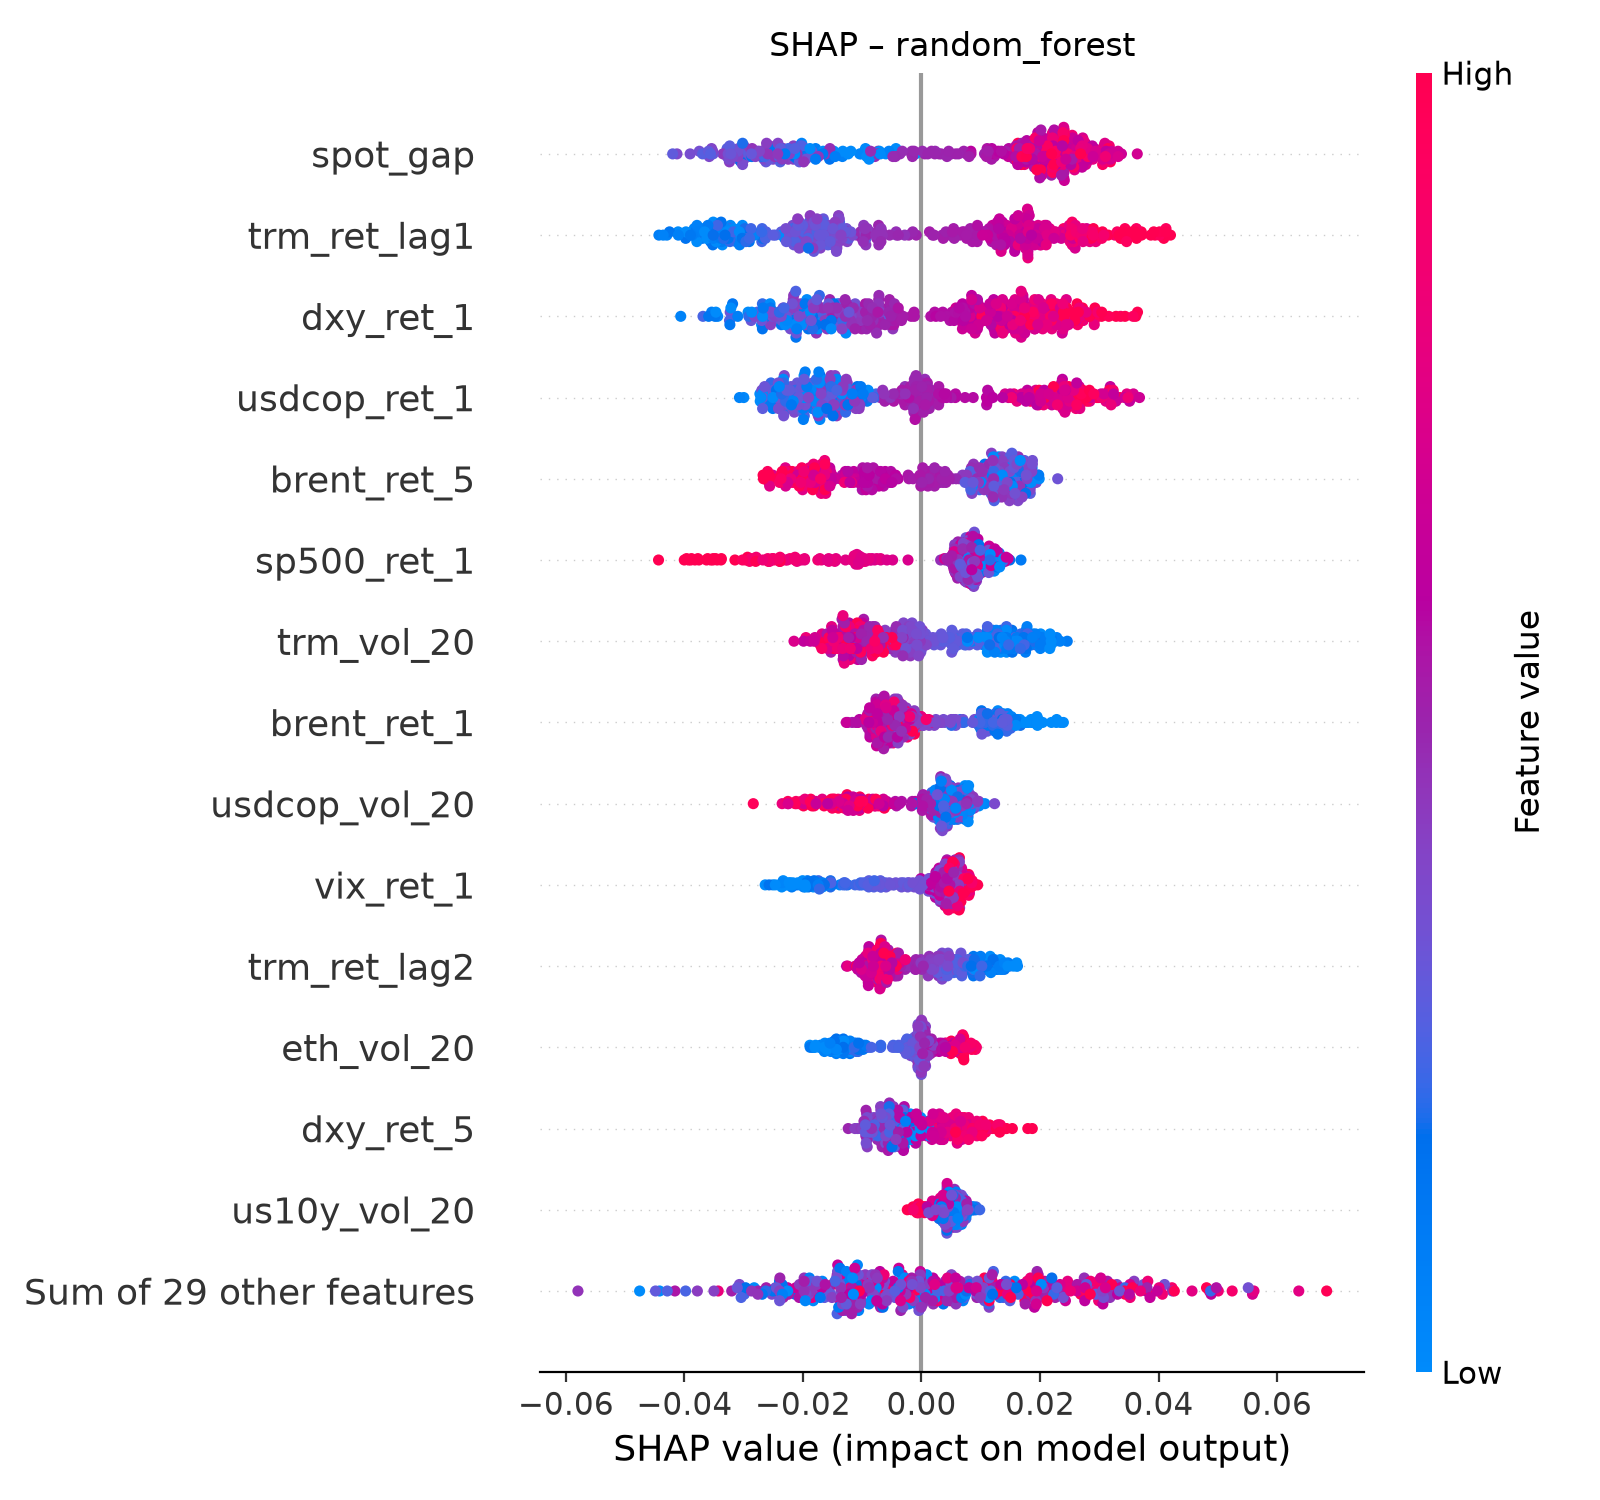
\includegraphics[width=0.92\columnwidth]{shap_beeswarm.png}
\caption{SHAP values of the Random Forest direction model on the test set.}
\label{fig:shap}
\end{figure}

\subsection{Decision-Oriented Evaluation}
Statistical metrics do not say whether the model helps a user. We simulated a household that receives USD~1{,}000 per day and either sells at the current TRM or waits one day when $P(\text{up})>\tau$. Over the test period (Fig.~\ref{fig:backtest}), the Random Forest rule with $\tau=0.5$ earns on average 383 COP per day relative to always selling at once, and 624 COP with $\tau=0.55$; Gradient Boosting earns 495 and 1{,}832 COP, respectively. A random wait-or-sell decision \emph{loses} 1{,}383 COP per day, because the peso appreciated during the test period, and a perfect oracle would earn 9{,}994 COP. The gains are small but positive and robust to the threshold. For the risk alert, a probability threshold chosen on the last training fold so that the alert rate matches the historical frequency yields a test precision of 30.1\% versus a base rate of 22.5\% (lift 1.34) with 25.8\% recall. The Random Forest probabilities are slightly better calibrated than the base rate (Brier 0.247 vs.\ 0.249).

\begin{figure}[t]
\centering
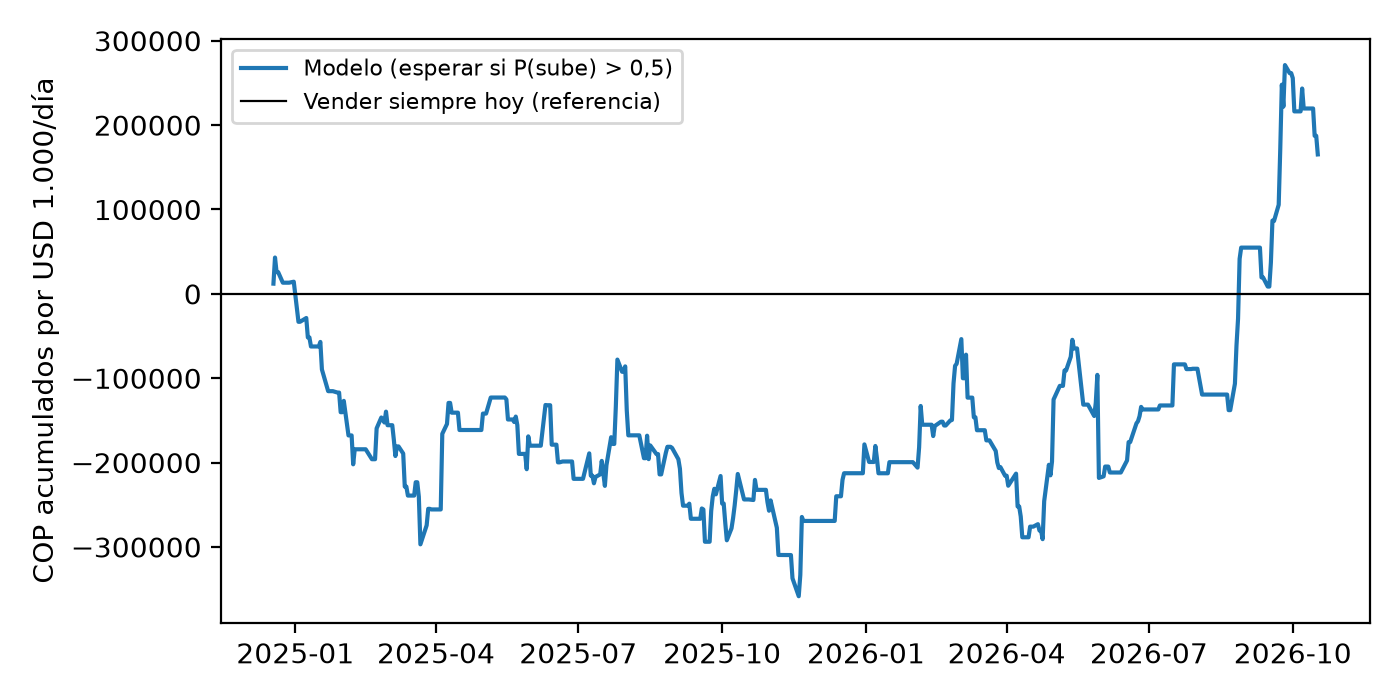
\includegraphics[width=\columnwidth]{decision_backtest.png}
\caption{Cumulative gain of the remittance-household rule (Random Forest, $\tau=0.5$) versus always selling immediately.}
\label{fig:backtest}
\end{figure}

\subsection{Model Selection}
Random Forest was selected for direction, risk and regression because it has the best cross-validation score in two of the three tasks, it is never far from the best test result, and a single model family simplifies maintenance and explanation. The randomized search of each ensemble takes 60--77~s on a laptop, and serving the three models takes about 0.5~s per request on a \texttt{t3.micro}. Gradient Boosting is kept as a documented alternative, as it reached slightly better test scores.

\section{Cloud Architecture and Deployment}
\subsection{Service and Deployment Models}
The system uses the public cloud of AWS (us-east-1) with a second region (us-west-2) for disaster recovery. Following NIST~\cite{nist800145}, it combines four service models (Table~\ref{tab:services}), each chosen for a reason: FaaS where work is sporadic, PaaS where state must be managed, and IaaS where the course requires explicit control of load balancing and auto-scaling.

\begin{table}[t]
\caption{Service models and justification}
\label{tab:services}
\centering
\footnotesize
\begin{tabular}{@{}p{1.0cm}p{2.3cm}p{4.1cm}@{}}
\toprule
Model & Service & Why \\
\midrule
FaaS & Lambda + EventBridge & Ingestion and ETL run seconds per day; paying per invocation is almost free \\
PaaS & RDS PostgreSQL & Managed backups, patches, Multi-AZ failover \\
PaaS & S3, ECR, ALB & Durable data lake, image registry, managed load balancing \\
IaaS & EC2 + Auto Scaling & Explicit control of instance type, scaling policy and health checks \\
SaaS & Web dashboard & Consumed by end users through a browser \\
\bottomrule
\end{tabular}
\end{table}

\subsection{Infrastructure as Code}
All infrastructure is declared in Terraform~\cite{terraform_aws} (10 files, 64 managed resources): VPC with public and private subnets in two availability zones, security groups, a free S3 gateway endpoint that replaces a NAT gateway, the versioned and encrypted data lake with lifecycle rules, cross-region replication, ECR, RDS, SSM parameters, ALB, launch template, Auto Scaling Group and target-tracking policy, both Lambdas with their triggers, CloudWatch alarms and dashboard, and a monthly AWS Budget. A single \texttt{terraform apply} creates the stack in about 15 minutes, most of them for RDS, and \texttt{terraform destroy} removes it. Variables allow the same code to run in AWS Academy, whose \texttt{LabRole} replaces the IAM roles that Terraform would otherwise create.

\subsection{Security}
RDS and the ETL Lambda live in private subnets without Internet egress; the database accepts connections only from the API and the ETL security groups; API instances accept traffic only from the ALB and require IMDSv2; the database password is generated by Terraform and stored encrypted in SSM Parameter Store; S3 blocks public access and encrypts at rest. No personal data are processed, so no informed consent is required.

\subsection{Scalability and High Availability: Experiments}
Two experiments were run against the deployed stack from a client in Colombia (Table~\ref{tab:exp}). Without load, \texttt{/health} answers in 197~ms (mostly network round trip), \texttt{/api/predict} in 709~ms and \texttt{/api/scenario} in 982~ms.

\emph{High availability.} A probe called \texttt{/health} every 0.5~s and one instance was terminated at $t=30$~s (Fig.~\ref{fig:ha}). In the first run the auto-scaling group had a minimum of one instance: because the idle group had already scaled in to a single server, terminating it left the load balancer without targets for about 109~s, until a replacement passed its health checks (availability 77.8\%). After raising the minimum to two (one per zone), the same test produced 378 successful requests out of 378; the load balancer drained the failed target and the group restored full capacity in 139~s. The lesson is that high availability depends on the scaling policy as much as on the multi-AZ topology.

\emph{Scalability.} Sixteen concurrent clients sent \texttt{POST /api/scenario} requests, the most CPU-intensive endpoint, for 14~min (Fig.~\ref{fig:load}). Target tracking at 60\% CPU raised the desired capacity from two to four at minute 6.6, and the new instances were healthy at minute 9.2. Throughput rose from 4.1 to 7.6 requests/s (+84\%) and the median latency fell from 4.0 to 1.6~s, with no errors in 4{,}543 requests. The roughly 2.5~min between the scaling decision and the new capacity is dominated by instance boot and image download, which a warm pool or a smaller image would shorten.

\begin{table}[t]
\caption{Results of the cloud experiments}
\label{tab:exp}
\centering
\footnotesize
\begin{tabular}{@{}lrrr@{}}
\toprule
\multicolumn{4}{@{}l}{\emph{High availability (one instance terminated)}} \\
ASG minimum & Availability & Outage & Recovery \\
\midrule
1 instance & 77.8\% & 109~s & --- \\
2 instances & 100\% & 0~s & 139~s \\
\midrule
\multicolumn{4}{@{}l}{\emph{Load test (16 clients, 4{,}543 requests, 0 errors)}} \\
Instances & Req/s & p50 (s) & p95 (s) \\
\midrule
2 & 4.12 & 4.05 & 7.62 \\
4 & 7.59 & 1.61 & 4.87 \\
\bottomrule
\end{tabular}
\end{table}

\begin{figure}[t]
\centering
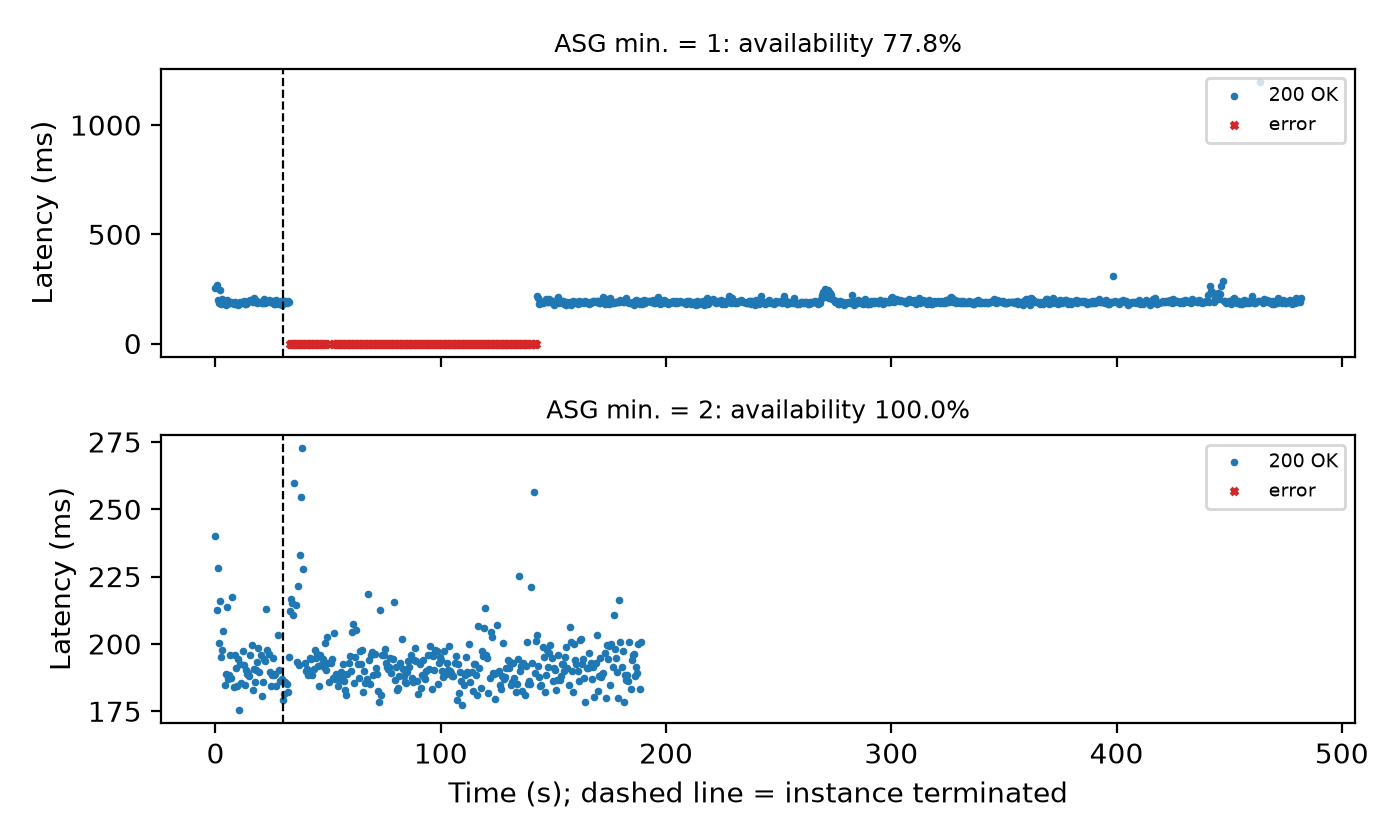
\includegraphics[width=\columnwidth]{ha_timeline_en.png}
\caption{Latency of \texttt{/health} probes when one instance is terminated (dashed line) with an ASG minimum of one (top) and two (bottom). Red crosses are failed requests.}
\label{fig:ha}
\end{figure}

\begin{figure}[t]
\centering
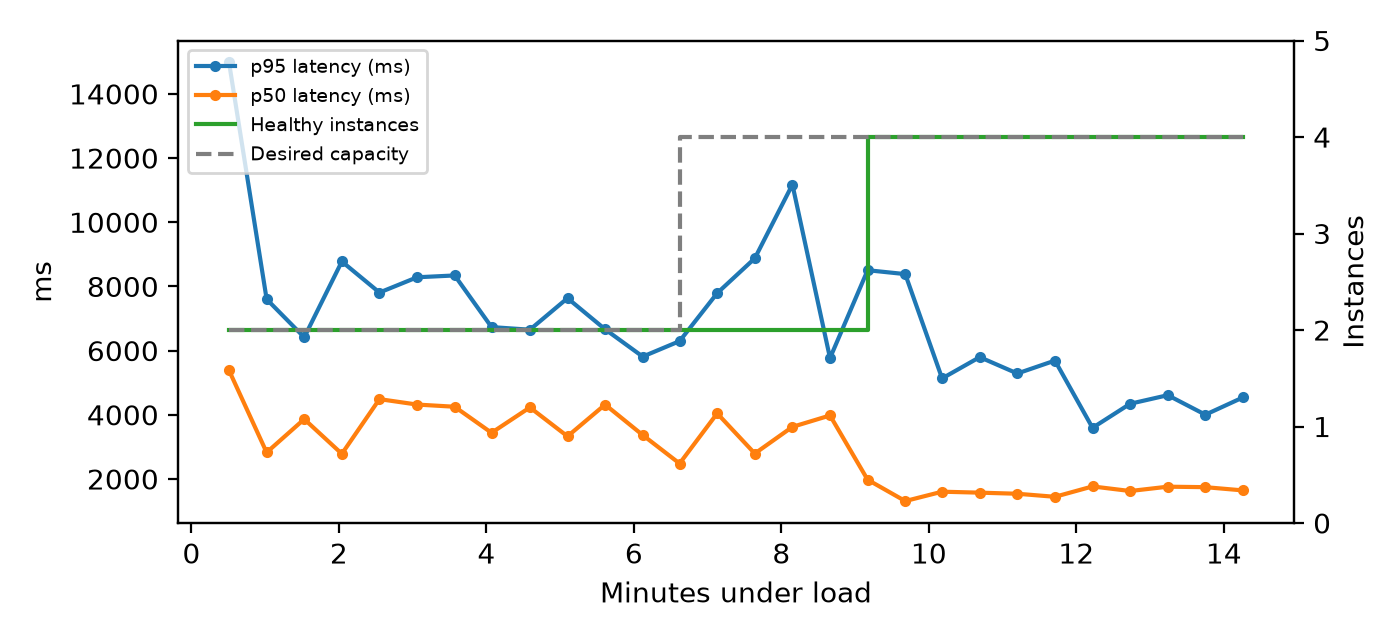
\includegraphics[width=\columnwidth]{load_timeline_en.png}
\caption{Load test: p50 and p95 latency, desired capacity and healthy instances. Latency drops once the two new instances pass their health checks.}
\label{fig:load}
\end{figure}

\subsection{Disaster Recovery}
S3 versioning protects against accidental deletion, and cross-region replication copied the 1.6~MB historical bundle and the 12~MB model to us-west-2 within minutes. RDS keeps seven days of automated backups with point-in-time recovery. Since all data can be re-ingested from public sources and all infrastructure is code, the strategy is \emph{backup and restore}~\cite{aws_wellarchitected} with RPO $\approx$ 24~h and RTO $<$ 1~h: \texttt{terraform apply} with \texttt{region=us-west-2} recreates the stack and the backfill reloads the database in about 2 minutes (14~s ingestion and 109~s ETL measured).

\subsection{Cost Analysis}
Table~\ref{tab:cost} compares the on-demand estimate with the observed usage. The dominant costs are the ALB, the public IPv4 addresses and the always-on EC2 and RDS instances; S3, Lambda, EventBridge and SSM are negligible. Avoiding a NAT gateway saves about USD~33 per month. Because the stack is created and destroyed with Terraform, the expected cost of the whole semester (about 40 development hours, one day of tests and one week of operation for the defense) is about USD~21. The deployment used for the experiments ran for about two days at an estimated USD~2 per day; AWS Cost Explorer reports charges with a delay of about 24~h, so the billed amount is added to the repository (\texttt{docs/costos.md}) once it is consolidated.

\begin{table}[t]
\caption{Monthly cost estimate (USD, on-demand, us-east-1, 24/7)}
\label{tab:cost}
\centering
\footnotesize
\begin{tabular}{@{}lr@{}}
\toprule
Service (configuration) & USD/month \\
\midrule
Application Load Balancer (low traffic) & 17.0 \\
EC2: 2 $\times$ t3.micro + 16 GB gp3 & 16.5 \\
Public IPv4 addresses (4) & 14.6 \\
RDS PostgreSQL db.t4g.micro + 20 GB & 14.0 \\
S3 + cross-region replica, ECR & 0.2 \\
Lambda, EventBridge, SSM & 0.0 \\
CloudWatch, data transfer & 1.3 \\
\midrule
\textbf{Total (dev, Single-AZ)} & \textbf{63.6} \\
Production (Multi-AZ, up to 4 instances) & 78--95 \\
Serverless alternative (API Gateway + Lambda) & $<$ 5 \\
\bottomrule
\end{tabular}
\end{table}

\section{Integration and Demo}
\begin{figure}[t]
\centering
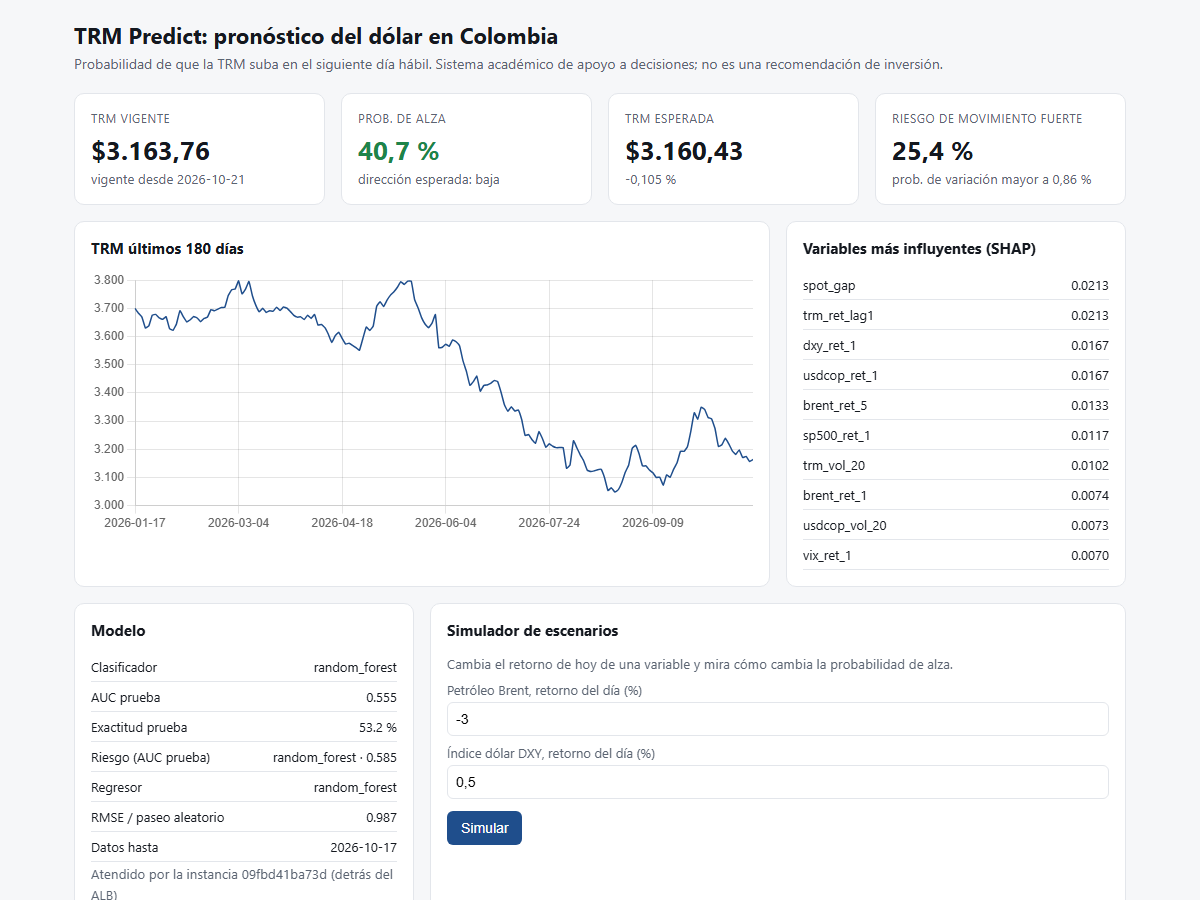
\includegraphics[width=\columnwidth]{tablero_aws.png}
\caption{Dashboard served from AWS: current TRM, probability of a rise, expected TRM, risk of a large move, SHAP drivers and the scenario simulator.}
\label{fig:dash}
\end{figure}

The deployed system works end to end: the historical backfill loaded 2{,}321 TRM records and 26{,}682 market observations into RDS, the daily schedule refreshes them after each publication, and the dashboard (Fig.~\ref{fig:dash}) and REST API (\texttt{/api/predict}, \texttt{/api/scenario}, \texttt{/api/history}, \texttt{/api/model}) answer from both availability zones. The \emph{scenario simulator} lets a user ask, for instance, how the probability of a rise changes if oil falls 3\% and the DXY rises 0.5\%. Code, data set, trained model and Terraform scripts are available in the public repository~\cite{repo}.

\section{Discussion and Limitations}
\label{sec:disc}
The results confirm the difficulty documented since Meese and Rogoff~\cite{meese1983}: the predictable component of daily FX moves is small and unstable. Three lessons follow. First, cross-validation alone was misleading: every model had a CV AUC near 0.56--0.58, but only the ensembles kept an edge on a later, unseen period; a strictly chronological test set was essential. Second, the most useful feature (spot--TRM gap) comes from domain understanding of how the TRM is computed rather than from model complexity. Third, decision-oriented metrics make modest statistical gains interpretable for users. Limitations: the test period was dominated by peso appreciation, so accuracy at the 0.5 threshold is below the majority class; the news-sentiment index lacks history; Yahoo Finance is an unofficial source; and the 2017 start date of crypto data shortens the sample.

\section{Conclusions and Future Work}
TRM Predict integrates a complete data-mining pipeline, an honestly evaluated set of machine-learning models and a scalable, highly available AWS architecture defined as code into one working product aligned with SDGs 8 and 10. Ensembles were the only models with out-of-sample value, and their signal translates into small but positive gains for a remittance household. Future work: probability calibration and cost-sensitive thresholds, adding the accumulated sentiment index and the policy-rate differential, walk-forward retraining scheduled in the cloud, and a serverless version of the API to cut the cost below USD~5 per month.

\begin{thebibliography}{99}
\bibitem{banrep_remesas} Banco de la Rep\'ublica de Colombia, ``Ingresos de remesas de trabajadores en Colombia,'' Estad\'isticas del sector externo, 2025. [Online]. Available: \url{https://www.banrep.gov.co}
\bibitem{un2015} United Nations, ``Transforming our world: The 2030 Agenda for Sustainable Development,'' A/RES/70/1, 2015.
\bibitem{meese1983} R. A. Meese and K. Rogoff, ``Empirical exchange rate models of the seventies: Do they fit out of sample?'' \emph{J. Int. Econ.}, vol. 14, no. 1--2, pp. 3--24, 1983.
\bibitem{henrique2019} B. M. Henrique, V. A. Sobreiro, and H. Kimura, ``Literature review: Machine learning techniques applied to financial market prediction,'' \emph{Expert Syst. Appl.}, vol. 124, pp. 226--251, 2019.
\bibitem{sezer2020} O. B. Sezer, M. U. Gudelek, and A. M. Ozbayoglu, ``Financial time series forecasting with deep learning: A systematic literature review: 2005--2019,'' \emph{Appl. Soft Comput.}, vol. 90, Art. no. 106181, 2020.
\bibitem{lundberg2017} S. M. Lundberg and S.-I. Lee, ``A unified approach to interpreting model predictions,'' in \emph{Adv. Neural Inf. Process. Syst. (NeurIPS)}, vol. 30, 2017, pp. 4765--4774.
\bibitem{ribeiro2016} M. T. Ribeiro, S. Singh, and C. Guestrin, ```Why should I trust you?': Explaining the predictions of any classifier,'' in \emph{Proc. 22nd ACM SIGKDD Int. Conf. Knowl. Discov. Data Min.}, 2016, pp. 1135--1144.
\bibitem{fayyad1996} U. Fayyad, G. Piatetsky-Shapiro, and P. Smyth, ``From data mining to knowledge discovery in databases,'' \emph{AI Mag.}, vol. 17, no. 3, pp. 37--54, 1996.
\bibitem{wirth2000} R. Wirth and J. Hipp, ``CRISP-DM: Towards a standard process model for data mining,'' in \emph{Proc. 4th Int. Conf. Pract. Appl. Knowl. Discov. Data Min.}, 2000, pp. 29--39.
\bibitem{ester1996} M. Ester, H.-P. Kriegel, J. Sander, and X. Xu, ``A density-based algorithm for discovering clusters in large spatial databases with noise,'' in \emph{Proc. 2nd Int. Conf. Knowl. Discov. Data Min. (KDD)}, 1996, pp. 226--231.
\bibitem{agrawal1994} R. Agrawal and R. Srikant, ``Fast algorithms for mining association rules,'' in \emph{Proc. 20th Int. Conf. Very Large Data Bases (VLDB)}, 1994, pp. 487--499.
\bibitem{han2000} J. Han, J. Pei, and Y. Yin, ``Mining frequent patterns without candidate generation,'' in \emph{Proc. ACM SIGMOD Int. Conf. Manag. Data}, 2000, pp. 1--12.
\bibitem{pedregosa2011} F. Pedregosa \emph{et al.}, ``Scikit-learn: Machine learning in Python,'' \emph{J. Mach. Learn. Res.}, vol. 12, pp. 2825--2830, 2011.
\bibitem{breiman2001} L. Breiman, ``Random forests,'' \emph{Mach. Learn.}, vol. 45, no. 1, pp. 5--32, 2001.
\bibitem{friedman2001} J. H. Friedman, ``Greedy function approximation: A gradient boosting machine,'' \emph{Ann. Statist.}, vol. 29, no. 5, pp. 1189--1232, 2001.
\bibitem{freund1997} Y. Freund and R. E. Schapire, ``A decision-theoretic generalization of on-line learning and an application to boosting,'' \emph{J. Comput. Syst. Sci.}, vol. 55, no. 1, pp. 119--139, 1997.
\bibitem{bergstra2012} J. Bergstra and Y. Bengio, ``Random search for hyper-parameter optimization,'' \emph{J. Mach. Learn. Res.}, vol. 13, pp. 281--305, 2012.
\bibitem{nist800145} P. Mell and T. Grance, ``The NIST definition of cloud computing,'' NIST, Gaithersburg, MD, USA, Special Publication 800-145, 2011.
\bibitem{terraform_aws} HashiCorp, ``Terraform AWS provider documentation,'' 2026. [Online]. Available: \url{https://registry.terraform.io/providers/hashicorp/aws/latest/docs}
\bibitem{aws_wellarchitected} Amazon Web Services, ``Disaster recovery of workloads on AWS: Recovery in the cloud,'' AWS Whitepaper, 2021. [Online]. Available: \url{https://docs.aws.amazon.com/whitepapers/latest/disaster-recovery-workloads-on-aws/}
\bibitem{repo} S. Cubides, N. Vergara, and E. Ruiz, ``TRM Predict,'' GitHub repository, 2026. [Online]. Available: \url{https://github.com/Sebas-409/proyecto-integrador-trm}
\end{thebibliography}

\end{document}
